
%(BEGIN_QUESTION)
% Copyright 2005, Tony R. Kuphaldt, released under the Creative Commons Attribution License (v 1.0)
% This means you may do almost anything with this work of mine, so long as you give me proper credit

Define what ``integral'' means when applied to the graph of a function.  For instance, examine this graph:

$$\includegraphics[width=15.5cm]{i01561x01.eps}$$

Sketch an approximate plot for the integral of this function.

\underbar{file i01561}
%(END_QUESTION)





%(BEGIN_ANSWER)

The graphical interpretation of ``integral'' means the {\it area} accumulated underneath the function for a given domain.

$$\includegraphics[width=15.5cm]{i01561x02.eps}$$

$$\includegraphics[width=15.5cm]{i01561x03.eps}$$

%(END_ANSWER)





%(BEGIN_NOTES)

Usually students find the concept of the integral a bit harder to grasp than the concept of the derivative, even when interpreted in graphical form.  One way to help them make this ``leap'' is to remind them that integration and differentiation are inverse functions, then ask them to analyze the answer ``backwards'' (looking at the red integral plot and seeing how the blue function is the derivative of the red function).  The thought process is analogous to explaining logarithms to students for the very first time: when we take the logarithm of a number, we are figuring out what power we would have to raise the base to get that number (e.g. $\log 1000 = 3$ ; $10^3 = 1000$).  When we determine the integral of a function, we are figuring out what other function, when differentiated, would result in the given function.  This is the essence of what we mean by {\it inverse functions}, and it is an important concept in algebra, trigonometry, and calculus alike.

%INDEX% Mathematics, calculus: integral (defined in a graphical sense)

%(END_NOTES)


